% Generated by pysimcount.pffig13 -- do not edit; regenerate instead.
% figure: fig13-rz -- Replica of Childs et al. 2018 Fig. 13 right: Rz before/after optimisation, Suzuki orders, empirical bound (Eq. 147)
% metric=rz gatebase=cz unmerged (simcount template); r_method=emp: r = Eq. 147 (Childs et al.'s power-law fit on n = 5-12, extrapolated to these n), not our measured r
% formulas: Lie-Trotter S1, Suzuki S2, Suzuki S4, Suzuki S6, Suzuki S8
% after = pysimcount.nam Light reconstruction, r x marginal + edge; verified for n <= 16 only
% before equals simcount's published pre-optimisation circuits (pf4emp, pf6emp) at every n
% figure made at git_commit=e5d9ee696f892e28aced765585653760f8a427c4 git_dirty=False
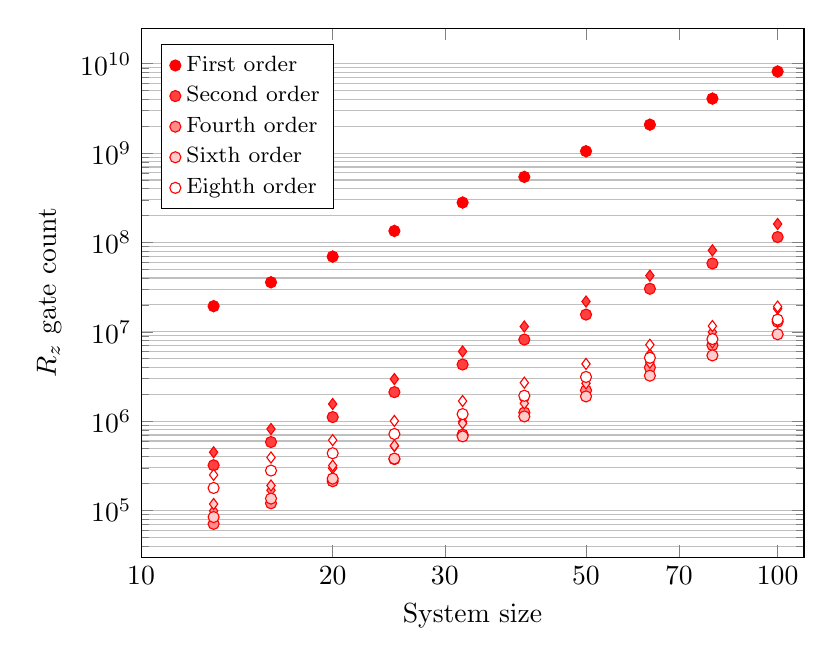
\begin{tikzpicture}
  \begin{loglogaxis}[
    width=10cm, height=8.3cm,
    xlabel={System size}, ylabel={$R_z$ gate count},
    xmin=10, xmax=110,
    ymin=30000, ymax=2.5e+10,
    xtick={10,20,30,50,70,100}, xticklabels={10,20,30,50,70,100},
    ymajorgrids=true, yminorgrids=true,
    legend pos=north west, legend cell align=left,
    legend style={font=\footnotesize},
  ]
    \addplot[only marks, mark=*, mark size=2pt, draw=red, fill=red] coordinates {
      (13,19369532)
      (16,35843008)
      (20,69445920)
      (25,134551600)
      (32,279679488)
      (40,541880000)
      (50,1049894200)
      (63,2082788316)
      (79,4073499436)
      (100,8192232400)
    };
    \addlegendentry{First order}
    \addplot[only marks, mark=diamond*, mark size=2pt, draw=red, fill=red, forget plot] coordinates {
      (13,19369532)
      (16,35843008)
      (20,69445920)
      (25,134551600)
      (32,279679488)
      (40,541880000)
      (50,1049894200)
      (63,2082788316)
      (79,4073499436)
      (100,8192232400)
    };
    \addplot[only marks, mark=*, mark size=2pt, draw=red, fill=red!75] coordinates {
      (13,320918)
      (16,583856)
      (20,1110920)
      (25,2113525)
      (32,4305792)
      (40,8192240)
      (50,15587050)
      (63,30345273)
      (79,58266134)
      (100,114953100)
    };
    \addlegendentry{Second order}
    \addplot[only marks, mark=diamond*, mark size=2pt, draw=red, fill=red!75, forget plot] coordinates {
      (13,449267)
      (16,817376)
      (20,1555260)
      (25,2958900)
      (32,6028064)
      (40,11469080)
      (50,21821800)
      (63,42483294)
      (79,81572477)
      (100,160934200)
    };
    \addplot[only marks, mark=*, mark size=2pt, draw=red, fill=red!45] coordinates {
      (13,70863)
      (16,120416)
      (20,212520)
      (25,376275)
      (32,706432)
      (40,1249040)
      (50,2207550)
      (63,3983238)
      (79,7102179)
      (100,12967600)
    };
    \addlegendentry{Fourth order}
    \addplot[only marks, mark=diamond*, mark size=2pt, draw=red, fill=red!45, forget plot] coordinates {
      (13,99190)
      (16,168560)
      (20,297500)
      (25,526750)
      (32,988960)
      (40,1748600)
      (50,3090500)
      (63,5576445)
      (79,9942940)
      (100,18154500)
    };
    \addplot[only marks, mark=*, mark size=2pt, draw=red, fill=red!20] coordinates {
      (13,84513)
      (16,136016)
      (20,227520)
      (25,381275)
      (32,676032)
      (40,1130040)
      (50,1893800)
      (63,3228813)
      (79,5441204)
      (100,9387600)
    };
    \addlegendentry{Sixth order}
    \addplot[only marks, mark=diamond*, mark size=2pt, draw=red, fill=red!20, forget plot] coordinates {
      (13,118300)
      (16,190400)
      (20,318500)
      (25,533750)
      (32,946400)
      (40,1582000)
      (50,2651250)
      (63,4520250)
      (79,7617575)
      (100,13142500)
    };
    \addplot[only marks, mark=*, mark size=2pt, draw=red, fill=white] coordinates {
      (13,178763)
      (16,280016)
      (20,437520)
      (25,718775)
      (32,1200032)
      (40,1925040)
      (50,3125050)
      (63,5118813)
      (79,8295079)
      (100,13687600)
    };
    \addlegendentry{Eighth order}
    \addplot[only marks, mark=diamond*, mark size=2pt, draw=red, fill=white, forget plot] coordinates {
      (13,250250)
      (16,392000)
      (20,612500)
      (25,1006250)
      (32,1680000)
      (40,2695000)
      (50,4375000)
      (63,7166250)
      (79,11613000)
      (100,19162500)
    };
  \end{loglogaxis}
\end{tikzpicture}
